\documentclass[12pt]{article}
\usepackage[paper=letterpaper,margin=2cm]{geometry}
\usepackage{amsmath}
\usepackage{amssymb}
\usepackage{amsfonts}
\usepackage{newtxtext, newtxmath}
\usepackage{enumitem}
\usepackage{titling}
\usepackage[colorlinks=true]{hyperref}
\usepackage{graphicx}
\usepackage{float}
\usepackage{listings}
\usepackage{xcolor}
\usepackage{color}
\usepackage{caption}
\usepackage{subfigure}
\definecolor{dkgreen}{rgb}{0,0.6,0}
\definecolor{gray}{rgb}{0.5,0.5,0.5}
\definecolor{mauve}{rgb}{0.58,0,0.82}
\lstset{ %
        language=Java,                
  basicstyle=\footnotesize,     
  numbers=left,               
  numberstyle=\tiny\color{gray},
  stepnumber=1,                                       
  numbersep=5pt,                 
  backgroundcolor=\color{white},  
  showspaces=false,             
  showstringspaces=false,         
  showtabs=false,                 
  frame=single,                   
  rulecolor=\color{black},       
  tabsize=4,                   
  captionpos=b,        
  breaklines=true,             
  breakatwhitespace=false,       
  title=\lstname,                                                  
  keywordstyle=\color{blue},          
  commentstyle=\color{dkgreen},    
  stringstyle=\color{mauve},       
  escapeinside={\%*}{*},        
  morekeywords={*,...}
} 

\setlength{\droptitle}{-6em}

% Enter the specific assignment number and topic of that assignment below, and replace "Your Name" with your actual name.
\title{Assignment 3: Comp 6771 Image Processing}
\author{Yunqi Xu 40130514}
\date{\today}



\begin{document}
% \maketitle

\begin{titlepage}
  \rule{\textwidth}{1pt}   % The top horizontal rule
    \vspace{0.2\textheight}  % Whitespace between top horizontal rule and title

    %------------------------------------------------------------
    %    Title
    %------------------------------------------------------------

    {\Huge COMP 6771 Image Processing: Assignment 2}

    \vspace{0.025\textheight}   % Whitespace between the title and short horizontal rule

    \rule{0.83\textwidth}{0.4pt}  % The short horizontal rule under title

    \vspace{0.1\textheight}  % Whitespace between the short horizontal rule and author

    %------------------------------------------------------------
    %    Author
    %------------------------------------------------------------

    {\Large Student name: \textsc{Yunqi Xu}}
    \vfill
    {\Large Student id: 40130514}
    \vfill  % Whitespace between author and date

    {\large \today}
    \vspace{0.1\textheight}  % Whitespace between date and bottom horizontal rule

    %------------------------------------------------------------
    %    Bottom rules
    %------------------------------------------------------------

    \rule{\textwidth}{1pt}  % The bottom horizontal rule
\end{titlepage}

\section{Review}
\subsection{Review of Bilateral Filter}
% overall summary of bilateral filter
Bilateral Filter is one of the most important filter method which presented by Tomasi in 1998. 
The bilateral filter smoothing image and preserve edges information at the meanwhile.

% review of the bilateral filter method
The main method that the bilateral filter utilized are two Gaussian filters. 
One is calcualted based on the Geometric closeness. 
Another is calculated based on their photometric similarity
% achievement



\subsection{Review of another paper}
% In this section, first introduce another method that provided by other paper, and then compared with the Bilateral filter


\section{Re-impleement of Bilateral Filter}
In this section, we will firstly present the result of our re-implement method, and then compared the bilater filter with other baseline algorithm in terms of other low pass filters that usually blur the image but also blur edges


\subsection{Result of the Re-implement algorithm}
In this section, we will use the images in the paper[cite here] to show our result that has successfully achieve the main goal which introduced by the paper.

Firstly, we present our result compared with the result indicated in the paper, with the same inputted parameters and the same pattern.

\begin{figure}[htbp]
  \centering
  \subfigure[$\sigma_d=1, \sigma_r=10$]{
  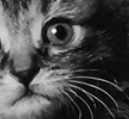
\includegraphics[width=3.5cm]{output_image/cat_part_ds1_rs10.png}
  % \caption{fig1}
  }
  \quad
  \subfigure[$\sigma_d=1, \sigma_r=30$]{
  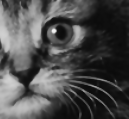
\includegraphics[width=3.5cm]{output_image/cat_part_ds1_rs30.png}
  }
  \quad
  \subfigure[$\sigma_d=1, \sigma_r=100$]{
  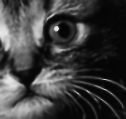
\includegraphics[width=3.5cm]{output_image/cat_part_ds1_rs100.png}
  }
  \quad
  \subfigure[$\sigma_d=1, \sigma_r=300$]{
  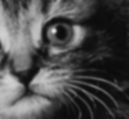
\includegraphics[width=3.5cm]{output_image/cat_part_ds1_rs300.png}
  }

  \subfigure[$\sigma_d=3, \sigma_r=10$]{
  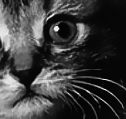
\includegraphics[width=3.5cm]{output_image/cat_part_ds3_rs10.png}
  % \caption{fig1}
  }
  \quad
  \subfigure[$\sigma_d=3, \sigma_r=30$]{
  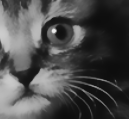
\includegraphics[width=3.5cm]{output_image/cat_part_ds3_rs30.png}
  }
  \quad
  \subfigure[$\sigma_d=3, \sigma_r=100$]{
  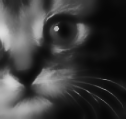
\includegraphics[width=3.5cm]{output_image/cat_part_ds3_rs100.png}
  }
  \quad
  \subfigure[$\sigma_d=3, \sigma_r=300$]{
  
\includegraphics[width=3.5cm]{output_image/cat_part_ds3_rs300.png}
  }

  \subfigure[$\sigma_d=10, \sigma_r=10$]{
  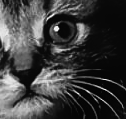
\includegraphics[width=3.5cm]{output_image/cat_part_ds10_rs10.png}
  % \caption{fig1}
  }
  \quad
  \subfigure[$\sigma_d=10, \sigma_r=30$]{
  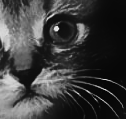
\includegraphics[width=3.5cm]{output_image/cat_part_ds10_rs30.png}
  }
  \quad
  \subfigure[$\sigma_d=10, \sigma_r=100$]{
  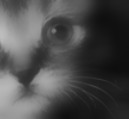
\includegraphics[width=3.5cm]{output_image/cat_part_ds10_rs100.png}
  }
  \quad
  \subfigure[$\sigma_d=10, \sigma_r=300$]{
  
\includegraphics[width=3.5cm]{output_image/cat_part_ds10_rs300.png}
  }
  \caption{A detail figure with bilateral filters with various range and domain parameter values by implement code}
  \end{figure}


\begin{figure}[htbp]
  \centering
  \subfigure[$\sigma_d=1, \sigma_r=10$]{
  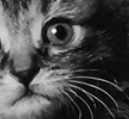
\includegraphics[width=3.5cm]{output_image/cat_part_ds1_rs10.png}
  % \caption{fig1}
  }
  \quad
  \subfigure[$\sigma_d=1, \sigma_r=30$]{
  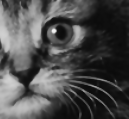
\includegraphics[width=3.5cm]{output_image/cat_part_ds1_rs30.png}
  }
  \quad
  \subfigure[$\sigma_d=1, \sigma_r=100$]{
  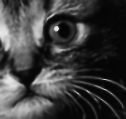
\includegraphics[width=3.5cm]{output_image/cat_part_ds1_rs100.png}
  }
  \quad
  \subfigure[$\sigma_d=1, \sigma_r=300$]{
  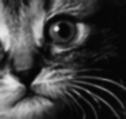
\includegraphics[width=3.5cm]{output_image_python/cat_part_ds1_rs300.png}
  }

  \subfigure[$\sigma_d=3, \sigma_r=10$]{
  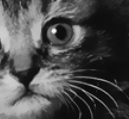
\includegraphics[width=3.5cm]{output_image_python/cat_part_ds3_rs10.png}
  % \caption{fig1}
  }
  \quad
  \subfigure[$\sigma_d=3, \sigma_r=30$]{
  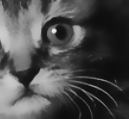
\includegraphics[width=3.5cm]{output_image_python/cat_part_ds3_rs30.png}
  }
  \quad
  \subfigure[$\sigma_d=3, \sigma_r=100$]{
  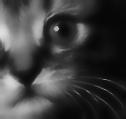
\includegraphics[width=3.5cm]{output_image_python/cat_part_ds3_rs100.png}
  }
  \quad
  \subfigure[$\sigma_d=3, \sigma_r=300$]{
  
\includegraphics[width=3.5cm]{output_image_python/cat_part_ds3_rs300.png}
  }

  \subfigure[$\sigma_d=10, \sigma_r=10$]{
  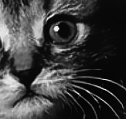
\includegraphics[width=3.5cm]{output_image_python/cat_part_ds10_rs10.png}
  % \caption{fig1}
  }
  \quad
  \subfigure[$\sigma_d=10, \sigma_r=30$]{
  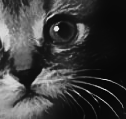
\includegraphics[width=3.5cm]{output_image_python/cat_part_ds10_rs30.png}
  }
  \quad
  \subfigure[$\sigma_d=10, \sigma_r=100$]{
  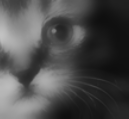
\includegraphics[width=3.5cm]{output_image_python/cat_part_ds10_rs100.png}
  }
  \quad
  \subfigure[$\sigma_d=10, \sigma_r=300$]{
  
\includegraphics[width=3.5cm]{output_image_python/cat_part_ds10_rs300.png}
  }
  \caption{A detail figure with bilateral filters with various range and domain parameter values by Opencv python}
  \end{figure}

The result indicates that our re-implement method of Bilateral filter can output the same grey result no matter compared with built-in opencv method or printed on paper.


\subsection{Compare with other baseline algorithm}
% in this section, compared with other blur algorithm

\end{document}
